\chapter{Background \label{sec:background}}

\section{Software Testing}
\label{sec:Testing}

Testing is a critical part of the software development life cycle \cite{testing}. It aims to minimize the risk of errors inside the software itself.
In testing, we attempt to determine whether the semantics of a software follows their specifications. However, we quote Dijkstra's famous line \cite{dahl_structured_1972}: 

\begin{quote}
    "Testing can be used to show the presence of bugs, but never to show their absence".
\end{quote}

\subsection{Regression Testing}

In software engineering, the most commonly used method of software testing is regression testing. Regression testing revolves around 
identifying parts of the program that are changed and verifying their behavior through a test suite; e.g. Unit, System, and Integration-level tests
\cite{testing}. Thus, that should verify whether the program behaves \emph{as intended or not}.

In practice, regression testing is limited to the capabilities of humans to define the behavior of the program. Therefore, there is an inherent 
risk of errors happening due to human mistakes; as it's possible that the defined behavior is not correct. Defining the complete set of the behavior 
of the intended program through testing requires developers to spend a considerable amount of time writing tests manually \cite{differentialTesting}. 

Thus, \textbf{random testing} is introduced to substitute humans with defined systematic computer behaviors.

\subsection{Random Testing}

Random testing is a suite of random tests generated by the computer to determine the correctness of the program based on a predetermined 
set of rules \cite{differentialTesting}. For example, \cite[Sec. 2]{randomTesting} generates test cases and 
executes them on programs that have a predictable result. For instance, if a program deviates from the expected results, then the 
program has undefined behaviors.

The difficulty of random testing lies in determining the set of rules to generate test cases. In \cite{differentialTesting}, the test cases 
are generated by substituting the subset of the input to a random input. While this allows test cases to be generated quickly, programs would only 
need several \emph{"interesting values"} or edge cases to consider in their behavior. As such, a stronger test suite such as an 
\textbf{inference-based test generation} will be preferable in this project.

\subsection{Inference-based Exhaustive Testing}
\label{sec:inferenceTesting}

Exhaustive tests such as \cite{isabelleQuickcheck} take into account the possible variable bounds of a program and convert it to a set of 
inference rules. For a program to be correct, all of the premises \emph{(P, Q)} in the inference rules \emph{(P \rightarrow Q)} must be correct. Hence, 
finding a counterexample is as simple as determining if the bounds of a variable result in a satisfiable \emph{\lnot(P \rightarrow Q)}. 
This could be extended even further by checking the inference rules on an SAT solver to find premises where the inference rules are incorrect 
\cite[Ch. 5]{isabelleProof}. Exhaustive searching allows developers to only focus on defining the behavior of the program, rather than defining 
tests to define the behavior.

\subsection{Mutation Testing}
\label{sec:mutationTesting}

Mutation testing is a form of testing where faults (or mutations) are inserted into a program \cite{offutt_mutation_2006}. 
These mutations are based on the grammar of the program, and would represent programs that are invalid. A key aspect of mutation testing is to 
determine suitable mutations to inject into the program called \emph{mutation operators} \cite[Sec. 2]{offutt_mutation_2006}, 
as inserting random values into the program would be akin to random testing. Specifically, Offutt et al. \cite[Sec. 6]{offutt_mutation_2006} 
elaborates how mutation testing can be used to generate valid or invalid input strings that will have erroneous responses.

\begin{figure}[h]
    \begin{tabular}{|L{0.95\textwidth}|}
        \hline
        \begin{enumerate}
            \item \textbf{Nonterminal Replacement}
            
            Every nonterminal symbol in a production is replaced by other nonterminal symbols.
    
            \item \textbf{Terminal Replacement}
            
            Every terminal symbol in a production is replaced by other terminal symbols.
    
            \item \textbf{Terminal and Nonterminal Deletion}
            
            Every terminal and nonterminal symbol in a production is deleted.
    
            \item \textbf{Terminal and Nonterminal Duplication}
            
            Every terminal and nonterminal symbol in a production is duplicated.
        \end{enumerate} \\
        \hline
    \end{tabular}

    \caption{Mutation operators for input strings. Summarised from \cite[Sec. 6.2]{offutt_mutation_2006}}
    \label{fig:MutationOperators}
\end{figure}

\section{Formal Verification of Compiler}
\label{sec:verification}

If software code is the recipe for system behaviors, then a compiler would be the chef who puts it all together. Most people would assume that 
the behavior of compiled programs will match the input program exactly. However, this is usually not the case \cite{compcertVerification}. 
Chefs have their way of creating magical concoctions from a recipe, and so does a compiler. Not only does a compiler try to replicate 
system behaviors, but it will try to make them faster in their ways; i.e. adding optimizations or reducing unneeded behaviors. However, the 
original behavior of the program must be preserved in order to consider a compiler to be correct 
\cite{compcertVerification,AliveInLean,Alive2,Term_Graph_Optimizations}.

Verifying compiler correctness is not easy. While the correctness of software \emph{could} be verified by defining behaviors through 
regression testing, compiler bugs are infamous for being hard to spot \cite{testing, compcertVerification}. Hence, it will be time-consuming to 
do and not exactly productive. There are a multitude of ways that a compiler can go wrong \cite[Sec. 1.2]{CompilerOptimization}; 
all of which have their specific way of verification. 

For example, CompCert \cite{compcertVerification} tries to tackle all of the implementation and semantics errors inside a compiler 
(See Sec. \ref{sec:CompCert}) -- creating a completely verified compiler for the C language platform. Formally verifying compilers on the scale of 
CompCert will require vast amounts of time and resources, which projects often don't have.

As such, there are smaller-scale projects such as Alive \cite{AliveInLean} \& Alive2 \cite{Alive2} that focus on behavior translation errors 
in LLVM's peephole optimizer (See Sec. \ref{sec:Alive}). Veriopt attempts to work on the same steps as CompCert -- by defining the IR of GraalVM and 
proving much of the side-effect-free data-flow behavior optimizations that occur in GraalVM 
\cite{ATVA21_GraalVM_IR_Semantics,Term_Graph_Optimizations} (See Sec. \ref{sec:Veriopt}).

\subsection{CompCert}
\label{sec:CompCert}

CompCert verifies that Clight, a subset of the C programming language \cite{compcertVerification}, is correct through several steps:
\begin{enumerate}
    \item 
    With deterministic programs, a compiler compiles a source program to the produced program -- in which both of the programs must have 
    the same behavior.
    
    This step is done by augmenting the compiler code with a \emph{certificate} -- code that carries proof that the behavior is exactly as intended 
    \cite[Sec. 2.2]{compcertVerification}.

    \item Compiler optimization rules must be accompanied by the formal definition of their Intermediate Representation (IR) semantics 
          \cite{compcertVerification,ATVA21_GraalVM_IR_Semantics}.
    
    \item Lastly, to formally verify each of the optimization rules, a compiler must either:
    \begin{enumerate}
        \item
        Prove that the code implementing the optimization is correct \cite[Sec. 2.4]{compcertVerification}.
        
        Veriopt uses this approach in verifying data-flow optimizations (See Sec. \ref{sec:Veriopt}).

        \item 
        Prove that the unverified code produces the correct behavior in their translation \cite[Sec. 2.4]{compcertVerification}.

        Alive uses this approach in verifying LLVM (See Sec. \ref{sec:Alive}).
    \end{enumerate}
\end{enumerate}

CompCert formally verifies each step in the source, intermediate, and target languages that go through the compiler 
\cite[Sec. 3.3]{compcertVerification}. Furthermore, each code translation and optimization are accompanied by \emph{certificates} that prove 
the correctness of the semantics. This is done through Coq, a proof assistant similar to Isabelle. The workflow of Coq also remains closely related to 
Isabelle (See Sec. \ref{sec:Isabelle}) \cite[Sec. 3.3]{compcertVerification}. 

CompCert utilizes Coq not only to formally verify the semantics of Clight but also to generate the verified parts of the compiler code 
\cite[Sec. 3.4]{compcertVerification}. The clever part of CompCert is that it utilizes the functional programming capabilities of Coq 
to automatically generate code. As such, it is able to write a compiler-compiler -- which is the 3\textsuperscript{rd} step of compiler verification research 
\cite{CompilerOptimization}.

The formal verification of Clight results in 42000 lines of Coq -- approximately equivalent to 3 years of man-hours 
of work \cite[Sec. 3.3]{compcertVerification}. As you can see, replicating the results of CompCert will require an enormous amount of work.
Formal verifications such as Alive (See Sec. \ref{sec:Alive}) and Veriopt (See Sec. \ref{sec:Veriopt}) undertake the smaller subset, 
namely the 1\textsuperscript{st} and 2\textsuperscript{nd} step, of the compiler verification research thread \cite{CompilerOptimization}.

\subsection{Alive}
\label{sec:Alive}

Alive takes on a subset of compiler verification by verifying that code optimizations inside LLVM are correct \cite{AliveInLean}. For example, 
a compiler will optimize:

\begin{equation}
    (LHS\ =\ x\ *\ 2)\ \Longrightarrow\ (RHS\ =\ x\ <<\ 1)
    \label{eq:AliveTransformation}
\end{equation}

(\ref{eq:AliveTransformation}) explains that \(LHS\) is transformed into \(RHS\) \cite[Sec. 2.1]{AliveInLean}.
While this may seem trivial, there would be a lot of edge cases where the behavior translation might be incorrect (e.g., buffer overflows).

\begin{figure}[ht]
    \centering
    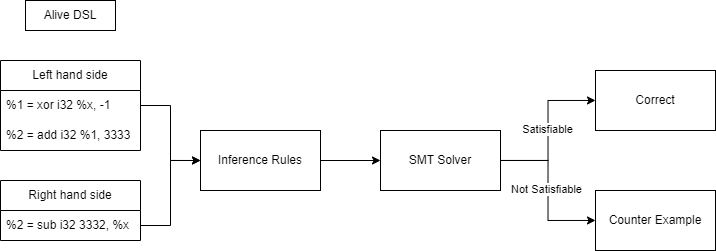
\includegraphics[width=1\textwidth]{Alive.png}
    \caption{How Alive verifies \((LHS\ =\ (X \oplus -1)\ +\ C) \Longrightarrow \ (RHS\ =\ (C-1)\ -\ X)\) \cite[p. 1]{AliveInLean}}
    \label{fig:AliveSystem}
\end{figure}

To verify that code optimizations are correct, Alive utilizes inference-based exhaustive testing (See Sec. \ref{sec:inferenceTesting}) that allows 
the tool to encode machine code behaviors to inference rules \cite[Sec. 3.1.1]{AliveInLean}. These inference rules are then passed to SMT solvers 
to check for their satisfiability (See Fig. \ref{fig:AliveSystem}). If the translation is proven to be correct, then it means that the underlying 
optimization code is correct.

Alive encodes LLVM's \cite{llvm} underlying IR semantics through their DSL \cite[Fig. 1]{AliveInLean}. The DSL specification is made to be 
similar to LLVM's IR semantics to allow developers to easily integrate Alive with the development of DSL. This represents the 
\emph{certificate} that the underlying optimization is formally verified to be correct.

Alive takes this further by creating Alive2: a system to translate LLVM IR into Alive's IR \cite{Alive2}. This allows the developers to entirely 
focus on developing LLVM, while completely ignoring the specifications of Alive. This is found to be effective, as differential testing of 
LLVM's unit tests and Alive2 discover multiple errors inside the unit test behaviors themselves \cite[Sec. 8.2]{Alive2}. Alive \& Alive2 covers 
the whole 1\textsuperscript{st} and 2\textsuperscript{nd} steps of the compiler optimization research thread \cite[p. 5]{CompilerOptimization}.

\section{Isabelle}
\label{sec:Isabelle}

Isabelle is an interactive theorem prover that utilizes a multitude of tools for automatic proving -- similar to Coq, used by CompCert 
\ref{sec:CompCert}. Isabelle emphasizes breaking down a proof 
for a theorem toward multiple smaller goals that are achievable called tactics. Tactics are functions, written in the implementation of Isabelle, 
that work on a proof state \cite{isabelleProof}. Tactics either output a direct proof towards the goal or break them down into smaller sub-goals 
in a divide-and-conquer manner. These tactics work on the foundation that theory definitions can be modified into a set of inference rules that 
could be automatically reasoned with by the system.

Finding the right proving methods and arguments to utilize is one of the biggest issues for proving a theorem \cite{isabelleProof}. 
Many tools in Isabelle's arsenal can help the user progress towards their proof \cite{IsabelleHOL}. However, the most notable ones are 
Sledgehammer, Quickcheck, and Nitpick.

\todo[inline]{mention isabelle benchmark}

\subsection{Sledgehammer}
\label{sec:Sledgehammer}

Sledgehammer is one of the tools in Isabelle that \emph{could} automatically prove a theorem. It utilizes the set of inference rules as 
conjectures that can be cross-referenced with relevant facts (lemmas, definitions, or axioms) from Isabelle \cite[Sec. 3]{isabelleProof}. 
Afterward, Sledgehammer passes them into resolution prover and SMT solvers that try to solve it \cite[Sec. 3.3]{isabelleProof}. If reasonable 
proof is found, Sledgehammer reconstructs the inference rules back into a \emph{relatively} human-readable proof definition in the style of 
Isabelle/Isar \cite[Sec. 3.4]{isabelleProof}.

Utilizing Sledgehammer has been proven to be an effective method of theorem proving. Sledgehammer, combined with external SMT solvers, can 
solve 60.1\% of proof goals, with a 44.7\% success rate for non-trivial goals \cite[Sec. 6]{isabelleSledgehammerSMT}. Despite their 
potential, as Blanchette et al. note \cite[p. 2]{isabelleProof}:

\begin{quote}
    "\dots most automatic proof tools are helpless in the face of an invalid conjecture. Novices and experts alike can enter invalid formulas and 
    find themselves wasting hours (or days) on an impossible proof; once they identify and correct the error, the proof is often easy."
\end{quote}

To make it easier for users to avoid this trap, Isabelle complements the automatic theory proving with counterexample generators such as Quickcheck 
and Nitpick.

\subsection{Quickcheck}
\label{sec:Quickcheck}

Quickcheck is one of the counterexample generators in Isabelle. It works by utilizing the code generation features of Isabelle by translating 
conjectures into ML (or Haskell) code \cite{isabelleQuickcheck}. This allows Quickcheck to discover counterexamples quickly by assigning 
free variables on the code via random, exhaustive, or narrowing test data generators. However, this would also mean that Quickcheck is limited 
to \emph{executable} and \emph{some} well-defined unbounded proof definitions \cite{isabelleQuickcheck}.

Random testing of a conjecture assigns free variables with pseudo-random values \cite[Sec. 3.1]{isabelleQuickcheck}. This strategy tends to be fast, 
with the ability to generate millions of test cases within seconds. However, random testing could easily overlook obvious counterexamples. 
Furthermore, random testing is also limited to well-defined proof definitions \cite{isabelleQuickcheck}. As such, exhaustive and narrowing 
test data generators are more suitable for proof definitions that are non-trivial or have unbounded variables.

Exhaustive and narrowing test data generators systematically generate values up to their bounds \cite{isabelleQuickcheck}. 
However, exhaustive test data generators fail to find counterexamples of proofs that have unbounded variables. Narrowing test data generators 
improves it by evaluating proof definitions symbolically rather than taking variables at face value. This is possible due to 
term rewriting static analysis done on proof definitions \cite[Sec. 5]{isabelleQuickcheck}.

Based on observed results, Bulwahn notes that random, exhaustive, and narrowing testing are comparable in terms of performance; with 
exhaustive testing finding non-trivial counterexamples easily compared to random testing \cite[Sec. 7]{isabelleQuickcheck}. As much of  
proof definitions are defined over unbounded variables, exhaustive testing is the default option for Quickcheck.

\subsection{Nitpick}
\label{sec:Nitpick}

Nitpick is an alternative to find counterexamples for proof definitions. Instead of enumerating the bounds of free variables inside the 
system of Isabelle, Nitpick passes conjectures -- translation of proof definitions into inference rules -- into SAT solvers 
\cite[Sec. 5]{isabelleProof}. SAT solvers search for the premises that falsify the given conjecture. If a conjecture 
has bounds over finite domains, Nitpick will \emph{eventually} find the counterexample. Conjectures with unbounded variables will be partially 
evaluated \cite[Sec. 5.2]{isabelleProof}. However, it could not determine whether infinite bounds result in a satisfiable conjecture.

Nitpick and Quickcheck shouldn't be compared to one another. Instead, they are tools that should be used interchangeably to determine 
whether a conjecture will be possible to prove \cite{isabelleQuickcheck}. The performance of Nitpick is comparable to Quickcheck, with 
the addition that Nitpick can find counterexamples to proof definitions that are not executable within Isabelle's code generation 
\cite[Sec. 7]{isabelleQuickcheck}.

\subsection{Limitations}

It is worthy to note that Quickcheck has some limitations over arbitrary type definitions \cite[Sec. 3.1]{isabelleQuickcheck} 
and conditional conjectures \cite[Sec. 4]{isabelleQuickcheck}. For arbitrary type definitions, Quickcheck is unable to transform the conjectures 
into internal Isabelle datatypes. As such, users need to define a way to \emph{construct} their datatype, which would be used by Quickcheck 
to build test generators. For conditional conjectures, Quickcheck would evaluate the given conjectures with no regards to their premises 
\cite[Sec. 4]{isabelleQuickcheck}. As such, users would need to specify their own test generators that would take the premises into account 
\cite[Sec. 4.1]{isabelleQuickcheck}. Furthermore, this limitations extends to Nitpick. For (Co)inductive datatypes, Nitpick needs the user to 
properly define their encoding of (Co)inductive datatypes, and manually provide selectors/discriminators if Nitpick cannot automatically infer 
one \cite[Sec. 5.4]{isabelleProof}.

\section{Veriopt}
\label{sec:Veriopt}

In comparison to CompCert and Alive, the theoretical aspects of compiler verification are similar. GraalVM's IR is made up of two components: 
control-flow nodes and data-flow nodes; which are combined as a sea-of-nodes data structure \cite{ATVA21_GraalVM_IR_Semantics}. However, 
Veriopt's DSL only concerns the subset of GraalVM's IR, which is the side-effect-free data-flow nodes \cite{Term_Graph_Optimizations}.
Side-effect-free data-flow nodes are comparatively easier to prove and optimize, as it is considered to be defined -- as opposed to LLVM's undefined 
and poisoned variables \cite{Alive2}.

\begin{figure}[h]
    \textbf{optimization} \emph{InverseLeftSub: \((x\ -\ y)\ +\ y \longmapsto x\)}
    \begin{enumerate}
        \item \(trm(x)\ <\ trm(BinaryExpr\ BinAdd\ (BinaryExpr\ BinSub\ x\ y)\ y)\)
        \item \(BinaryExpr\ BinAdd\ (BinaryExpr\ BinSub\ x\ y)\ y \sqsupseteq x\)
    \end{enumerate}

    \caption{Sample of Veriopt's optimization rule and proof obligations DSL \cite[Fig. 3]{Term_Graph_Optimizations}}
    \label{fig:VerioptDSLSample}
\end{figure}

Fig. \ref{fig:VerioptDSLSample} defines the structure of the DSL for an optimization rule. Veriopt's DSL is implemented in Isabelle 
\cite{IsabelleHOL}, which represents optimization rules as inductive datatypes that allows efficient reasoning within Isabelle 
\cite[Sec. 3]{ATVA21_GraalVM_IR_Semantics} \cite{biendarra_ning_2024}. 
The \textbf{optimization} keyword represents the proof definition that must be proven in Isabelle. 
Note that 2 proof obligations must be met to consider that the side-effect-free optimization is correct: 
(1) proof that the optimization rule will terminate; (2) proof that each pass of the optimization rule will 
result in a refinement of the expression \cite{Term_Graph_Optimizations}. Note that these proofs need to be provided by users.

Currently, there are some tools that the developers of GraalVM could use to provide a \emph{certificate} for the compiler code 
\cite[Sec. 7]{Term_Graph_Optimizations}. A semi-automated approach exists in the form of source code annotations \cite[Sec. 5.1]{Term_Graph_Optimizations}.
However, this semi-automated approach is inadequate due to only matching if the optimization rules exists in Veriopt's current theory base without 
any logical reasoning done. Providing proof obligations for an optimization rule will be challenging for developers who are not 
\emph{experts} in program verification, as it requires the developers of GraalVM to be familiar with Isabelle -- something that ideally Veriopt 
would like to avoid. Similar tools such as Alive \cite{AliveInLean} are preferable. Hence, that is where this project contributes.